\documentclass[../main.tex]{subfiles}

\begin{document}
    \subsection{パイプラインストール} \label{ssec:stallImprove}

        \ref{sssec:stall}で述べている方法には、FPGAボード上で実装としたら、
        メモリとのやりとりが問題となるだろう。
        今回は全てシムレーション上で機能検証およびベンチマークを行ったため、
        メモリへの書き込みと読み込みには、半クロックサイクルでデータの扱いができるため、

        これはパイプラインストーリより、
        ステージストールと認識しても良いと思い、
        確かに、問題がないが、効率が悪いだけである。
        これを実装する時に、パイプラインの出力をワイヤだと認識してしまったことが、
        自分のミスであった。

        ここで、メモリへのアクセスが1クロックサイクル以上がかかるとしたら、
        全てのパイプラインストールが必要となっている。

        本プロセッサで実装パイプラインストールは少し変える必要がある。
        それは、ストール信号を受ける時、今レジスタが格納しているデータをそのまま
        出力しただけで解決できると考えられる。
        もちろん、ストール検出にはメモリアクセスの成功の検出という機能を
        追加すべきである。
        さらに、PCの値を一時的に停止しないといけない。

        \begin{figure}[h]
            \centering
            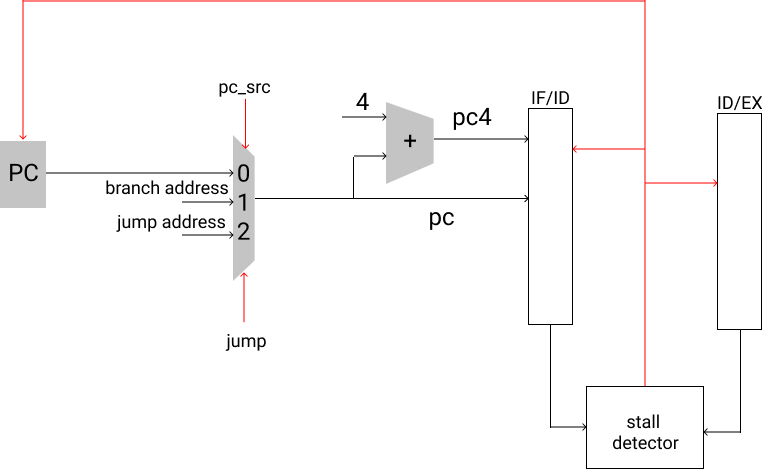
\includegraphics[width = 1.3\columnwidth]{../images/stall_improve.png}
            \caption{改善後のパイプラインストール}
            \label{fig:stallImprove}
        \end{figure}

    \subsection{クリティカルパースの短縮} \label{ssec:forwardingImprove}
        図\ref{fig:forwarding}を見れば、今のフォワーディング機がクリティカルパースになっているのは、
        パプラインに入る他の信号と比べたら、多少の論理ゲートを通過しないといけない
        パースになっているからだと考えられる。

        簡潔な方法としては、フォワーディング機をEXステージ持ち込めば、
        また、同じパースを作ることになるため、
        フォワーディングの原理を変えるべきだと考えられる。

        考えられる改善は\ref{fig:forwardingImprove}に示すように、
        ALUのあたりにマルチプレクサーとして実装し、
        フォワーディングの原理を含めば、EXステージのパースはあまり変わらず、
        クリティカルパースが短縮できると考えられる。

        \begin{figure*}[htp]
            \centering
            \includegraphics*[scale = 0.8]{../images/forwarding_improved.png}
            \caption{改善後フォワーディング}
            \label{fig:forwardingImprove}
        \end{figure*}
\end{document}
